\documentclass[letterpaper]{article} 

% \documentclass[]{article}



\usepackage{geometry}
\geometry{letterpaper, top=3.5cm, left=2cm, right=3.5cm, bottom=1.0cm}

\usepackage[compact]{titlesec}
\usepackage[document]{ragged2e}
\usepackage{multirow}
\usepackage{colortbl}

    \usepackage{lmodern}
    \usepackage{amssymb,amsmath}
\usepackage{ifxetex,ifluatex}
\usepackage{fixltx2e} % provides \textsubscript
\ifnum 0\ifxetex 1\fi\ifluatex 1\fi=0 % if pdftex
\usepackage[T1]{fontenc}
\usepackage[utf8]{inputenc}

\usepackage{color}


% pandoc syntax highlighting
  
    
% graphix
\usepackage{graphicx}
\setkeys{Gin}{width=\linewidth,totalheight=\textheight,keepaspectratio}

% booktabs
\usepackage{booktabs}

% float images
\usepackage{wrapfig}

\usepackage{array}


\usepackage[scaled]{helvet}
\renewcommand\familydefault{\sfdefault} 
\usepackage[T1]{fontenc}


\renewcommand{\arraystretch}{0}
\usepackage{ejbi}

\usepackage{fancyhdr}

\pagestyle{fancy}
\fancyhf{}
\fancyhead[LE,RO]{
\includegraphics[width=50mm]{logo.png}}

% \pagestyle{fancy}
% \fancyhf{}
% \fancyhead[R]{
\includegraphics[width=50mm]{logo.png}}
% \fancyfoot[R]{hola}
% % 
% % \setlength{\headheight}{10.50mm}
% \pagestyle{fancy}

\begin{document}



\begin{table}[h!]
 \setlength{\tabcolsep}{0pt}
\def\arraystretch{0}
  \begin{tabular}{m{4cm}m{12cm}}

    &
    \vspace{10pt} 

                \begin{center}
        \begin{ejbi-title}
        Las vías fantasma
        \end{ejbi-title}
        \end{center}
        %\bigskip
                      \begin{center}
      \begin{ejbi-subtitle}
      Empresa contratista en Santander recibió dinero para adelantar vías pero
      nunca las terminó
      \end{ejbi-subtitle}
      \end{center}
      %}
      %\bigskip
        \end{tabular}
%  \egroup
\end{table}


%\begin{abstract}
\color{colT}{\justify{2013, Santander, Corrupción Privada, Incumplimiento en Construcción de
vías}}
%\end{abstract}


\vspace{0.5cm}

\begin{center}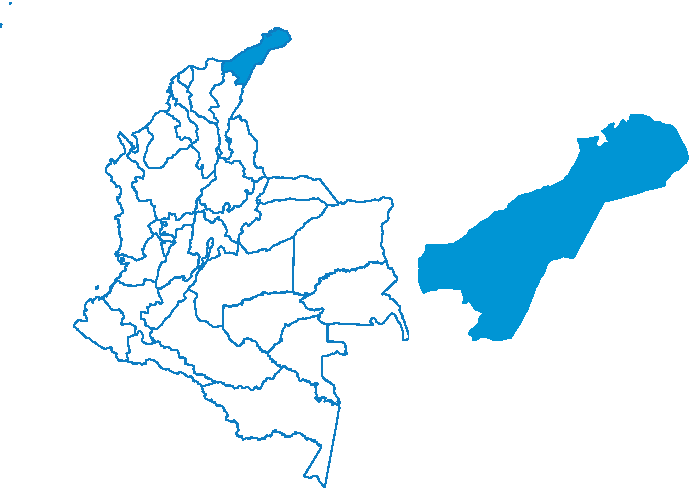
\includegraphics[width=150px,height=150px]{built_report_files/figure-latex/unnamed-chunk-3-1} \end{center}
  

  
\vspace{0.5cm}

\begin{minipage}[t]{0.45\textwidth}%
  
\begin{tabular}{m{3.4cm}m{3.6cm}}
 \begin{ejbi-colone}LUGAR DEL HECHO:\end{ejbi-colone}& 
  \begin{ejbi-coltwo} SANTANDER \end{ejbi-coltwo}\\ 
 \colrul 
 \addlinespace
 \begin{ejbi-colone}FECHA DE INICIO:\end{ejbi-colone} &
  \begin{ejbi-coltwo} 2013 \end{ejbi-coltwo}   \\
 \colrul 
 \addlinespace
 \specialcell[]{\begin{ejbi-colone}ACTOR O ENTIDAD\end{ejbi-colone} \\
 \addlinespace
 \begin{ejbi-colone}INVOLUCRADO: \end{ejbi-colone}}&
  \begin{ejbi-coltwo} Esgramo Ingenieros Constructores S.A.S \end{ejbi-coltwo} \\ 
\addlinespace\colrul
 \addlinespace
 \specialcell[]{\begin{ejbi-colone}TIPO DE \end{ejbi-colone}\\ 
 \begin{ejbi-colone}CORRUPCIÓN:\end{ejbi-colone}}&
  \begin{ejbi-coltwo} Corrupción Privada \end{ejbi-coltwo} \\
 \addlinespace \colrul
 \end{tabular}
\end{minipage}%
\qquad{\color{colfich}\vrule}\qquad
\begin{tabular}{@{}l@{}}

\begin{tabular}{m{3.6cm}m{3.6cm}}
\begin{ejbi-colone}DELITO\end{ejbi-colone} &
 \begin{ejbi-coltwo}Otros.\end{ejbi-coltwo}\\ 
\colrul
\addlinespace
\begin{ejbi-colone}SECTOR AFECTADO\end{ejbi-colone} &
 \begin{ejbi-colone}INFRAESTRUCTURA Y TRANSPORTE\end{ejbi-colone}\\ 
\colrul
\addlinespace
\multicolumn{1}{c !{\color{colfich}\vline}}{{\begin{tabular}{@{}c@{}}
 \\
 \\
 \begin{ejbi-colone}ENTIDAD DE\end{ejbi-colone}\\\addlinespace \begin{ejbi-colone}CONOCIMIENTO:\end{ejbi-colone}\end{tabular} }} & 
 \multicolumn{1}{c}{\begin{ejbi-colone}ESTADO JUDICIAL:\end{ejbi-colone}} 
 \\
 \multicolumn{1}{c !{\color{colfich}\vline}}{{\begin{ejbi-coltwo} \parbox[t]{3.4cm}{\begin{center}NA\end{center}}\end{ejbi-coltwo}}}  & \multicolumn{1}{c}{\begin{ejbi-coltwo}\parbox[t]{3.4cm}{\begin{center} Sanción Fiscal\end{center}} \end{ejbi-coltwo}} \\ \arrayrulecolor{colfich}\hline
\end{tabular}
\end{tabular}

\vspace{1cm}

\begin{flushright}
 \textit{Última actualización 2016} 
\end{flushright}

\end{document}




% 
% \begin{table}[h]
% \renewcommand\arraystretch{0.5}
% \centering
% \begin{tabular}{m{4cm}m{4cm}}
% \begin{ejbi-colone} LUGAR DEL HECHO: \end{ejbi-colone}& 
%  \begin{ejbi-coltwo} SANTANDER \end{ejbi-coltwo}\\ 
% \colrul 
%  \begin{ejbi-coltwo} 2013 \end{ejbi-coltwo}  & \begin{ejbi-coltwo} FECHA DE INICIO \end{ejbi-coltwo} \\
% \colrul 
% \specialcell[]{\begin{ejbi-colone}ACTOR O ENTIDAD \end{ejbi-colone} \\
% \begin{ejbi-colone} IMPLICADA: \end{ejbi-colone}} &
%  \begin{ejbi-coltwo} Esgramo Ingenieros Constructores S.A.S \end{ejbi-coltwo} \\ 
% \addlinespace\colrul
% \specialcell[]{\begin{ejbi-colone}TIPO DE \end{ejbi-colone}\\ 
% \begin{ejbi-colone}CORRUPCIÓN\end{ejbi-colone}}&
%  \begin{ejbi-coltwo} Corrupción Privada \end{ejbi-coltwo} \\
% \addlinespace \colrul
% \begin{ejbi-colone}DELITO\end{ejbi-colone} &
% \begin{ejbi-coltwo}Otros.\end{ejbi-coltwo}\\ 
% \colrul
% \multicolumn{2}{l}{\begin{tabular}[x]{@{}l@{}}\begin{ejbi-coltwo}DINERO \end{ejbi-coltwo}\\ \begin{ejbi-coltwo}EN JUEGO:\end{ejbi-coltwo}\end{tabular} } \\ 
% \addlinespace \arrayrulecolor{colfich}\hline
% \multicolumn{1}{c !{\color{colfich}\vline}}{{\begin{tabular}[x]{@{}c@{}} 
% \\
% \\
% \begin{ejbi-colone}ENTIDAD DE\end{ejbi-colone}\\\begin{ejbi-colone}CONOCIMIENTO:\end{ejbi-colone}\end{tabular} }} & 
% \multicolumn{1}{c}{\begin{ejbi-colone}ESTADO JUDICIAL:\end{ejbi-colone}} 
% \\
% \multicolumn{1}{c !{\color{colfich}\vline}}{{\begin{ejbi-coltwo} \parbox[t]{4cm}{\begin{center}NA\end{center}}\end{ejbi-coltwo}}}  & \multicolumn{1}{c}{\begin{ejbi-coltwo}\parbox[t]{4cm}{\begin{center} Sanción Fiscal\end{center}} \end{ejbi-coltwo}} \\ \arrayrulecolor{colfich}\hline
%         \end{tabular}
%     \end{table}